\documentclass{beamer}
%
% Choose how your presentation looks.
%
% For more themes, color themes and font themes, see:
% http://deic.uab.es/~iblanes/beamer_gallery/index_by_theme.html
%
\mode<presentation>
{
  \usetheme{Boadilla}      % or try Darmstadt, Madrid, Warsaw, ...
  \usecolortheme{beaver} % or try albatross, beaver, crane, ...
  \usefonttheme{default}  % or try serif, structurebold, ...
  \setbeamertemplate{navigation symbols}{}
  \setbeamertemplate{caption}[numbered]
  
} 

\usepackage{xcolor,colortbl}
\usepackage[english]{babel}
\usepackage[utf8x]{inputenc}
\usepackage{courier}
\usepackage{dsfont}
\usepackage{verbatim} 
\usepackage{enumerate}
\usepackage{tikz}
\usepackage{multirow}
\usepackage{venndiagram}
\usepackage{epigraph} 
%\usepackage{xcolor}

%\usepackage{enumitem}

\usepackage{hyperref}
\hypersetup{
    colorlinks=true,
    linkcolor=blue,
    filecolor=magenta,      
    urlcolor=cyan,
}

% R stuff!
\usepackage{listings}
\definecolor{codegreen}{rgb}{0,0.6,0}
\definecolor{codegray}{rgb}{0.5,0.5,0.5}
\definecolor{codepurple}{rgb}{0.58,0,0.82}
\definecolor{backcolour}{rgb}{0.95,0.95,0.92}

\lstdefinestyle{mystyle}{
    backgroundcolor=\color{backcolour},    
    commentstyle=\color{codegreen},
    keywordstyle=\color{black},
    numberstyle=\tiny\color{codegray},
    stringstyle=\color{codepurple},
    basicstyle=\ttfamily\footnotesize,
    breakatwhitespace=false,         
    breaklines=true,                 
    captionpos=b,                    
    keepspaces=true,                 
    numbers=left,                    
    numbersep=5pt,                  
    showspaces=false,                
    showstringspaces=false,
    showtabs=false,                  
    tabsize=2
}

\lstset{style=mystyle}


\setbeamertemplate{enumerate items}[default]
\setbeamertemplate{itemize item}[triangle]

%\setitemize{label=\usebeamerfont*{itemize item}%
%  \usebeamercolor[fg]{itemize item}
%  \usebeamertemplate{itemize item}}



\title[SST-115 / STA-209]{Simple Linear Regression}
\subtitle{}
\author{Grinnell College}
\date{September 25, 2024}

\graphicspath{{img/}}

\begin{document}

\begin{frame}
  \titlepage
\end{frame}

\begin{frame}{Review}
\begin{itemize}
    \item Scatterplot descriptions
        \begin{itemize}
            \item form, strength, direction
        \end{itemize} \vspace{3mm}
    \item Pearson's correlation (r)
        \begin{itemize}
            \item strength and direction of linear relationship for 2 quant. variables
        \end{itemize}\vspace{3mm}
    \item Spearman's correlation $(\rho)$
        \begin{itemize}
            \item strength and direction of \textit{monotone} relationship
            \item more robust to outliers
        \end{itemize}
\end{itemize}
\end{frame}



\begin{frame}{Basic Idea}
\textbf{Regression} is a technique that we can use when there is a linear relationship between 2 quantitative variables. \vspace{4mm}

\textbf{Regression} = creating a line on the scatterplot that best represents the linear relationship we see. \vspace{4mm}

\textbf{Goal}: use the explanatory variable to predict values for the response variable.
\begin{itemize}
    \item the variable being predicted is the response
    \item the variable we are using to predict is the explanatory variable ('predictor')
\end{itemize}
\end{frame}



\begin{frame}{Basic Idea}
We are going to create a line on the scatterplot that best represents the linear relationship we see. \vspace{4mm}

\fbox{\begin{minipage}{.9\textwidth}
\textbf{Algebra}

y = mx + b

m = slope: change in y over the change in x (rise / run)

b = intercept: value where the line cross the y-axis

All points fall exactly on the line
\end{minipage}} \vspace{4mm}

\fbox{\begin{minipage}{.9\textwidth}
\textbf{Statistics}

$\hat{y} = \beta_0 + \beta_1X$

$\beta_1$ = slope

$\beta_0$ = intercept

Not all of our data points will exactly on the line $\rightarrow$ variability
\end{minipage}}
\end{frame}



\begin{frame}{How it works}
Canidae data set (predicting bite force using body mass)
\begin{center}
    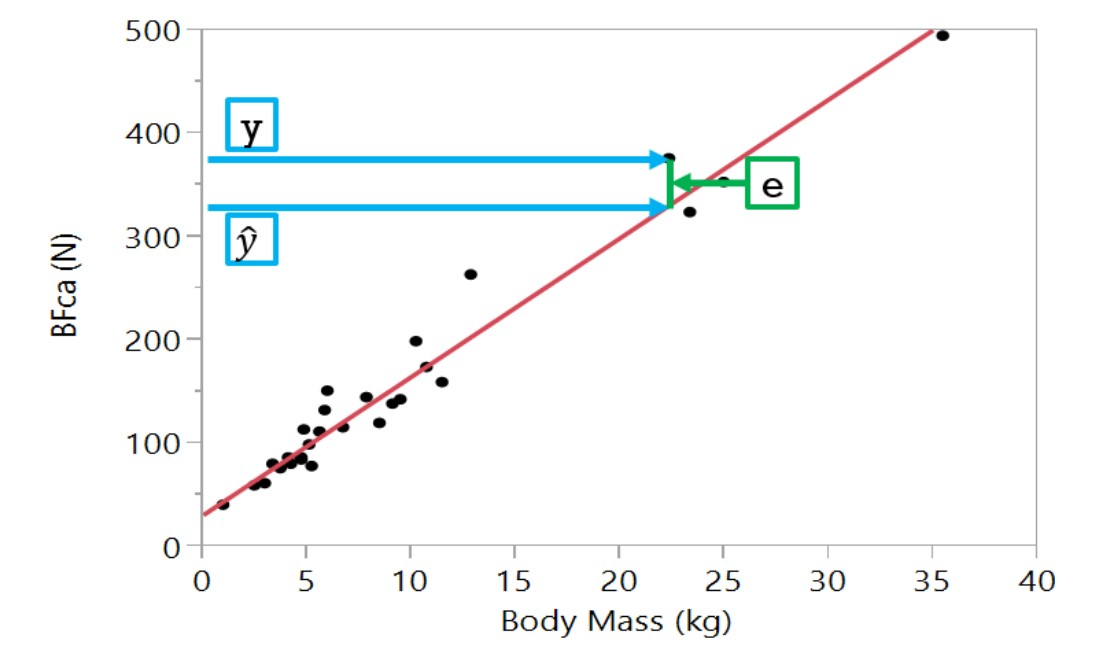
\includegraphics[scale=.4]{bite_force_regression_example.jpg}
\end{center}

The \textbf{regression line} is the line that fits through the data points.
\begin{itemize}
    \item y's denote the values of the datapoints for the response variable
    \item points on the line are predicted values for the y's, denoted as $\hat{y}$
    \item \textbf{residual}: difference between data and predictions (\textbf{e} = y - $\hat{y}$)
\end{itemize}
\end{frame}

\begin{frame}{How it works}
\begin{center}
    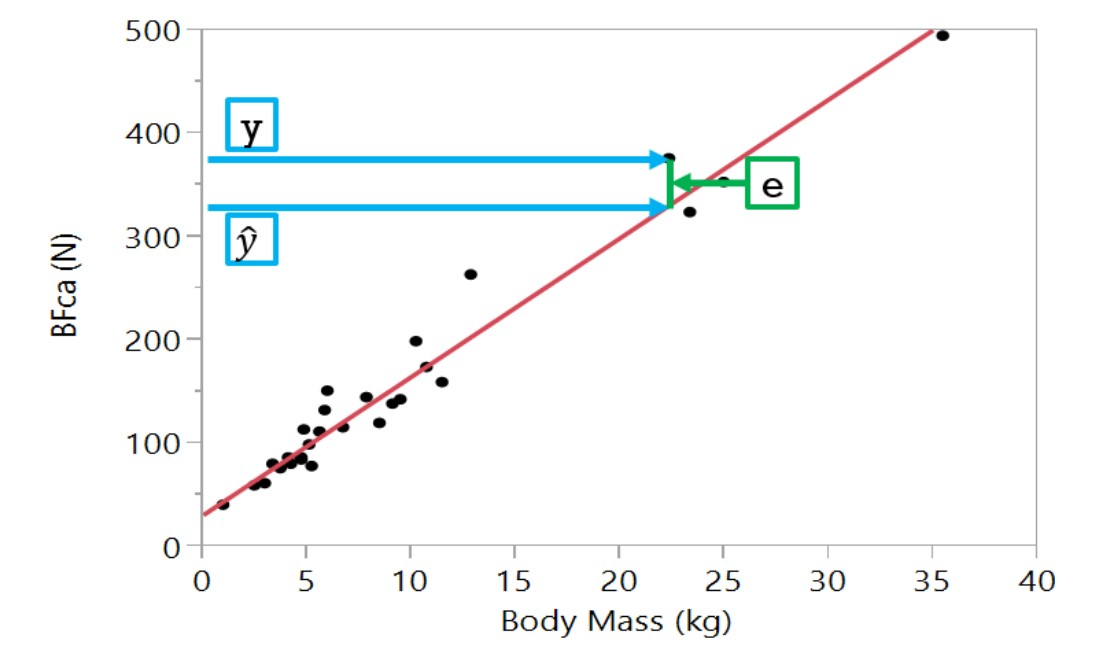
\includegraphics[scale=.3]{bite_force_regression_example.jpg}
\end{center}

The \textbf{regression line} is the line that best fits through the data
\begin{itemize}
    \item critera: minimizes sum of squared residuals $\sum e_i^2$
    \item $\hat{y} = b_0 + b_1X$ \hspace{2mm}(regression equation)
    \item $b_1 = (\frac{s_x}{s_y})r$ \hspace{2mm} (slope)
    \item $b_0 = \overline{y}-b_1 \overline{x}$ \hspace{2mm} (intercept)
\end{itemize}
\end{frame}



\begin{frame}{Pearson's Height Data}

\begin{table}[ht]
\centering
\footnotesize
\begin{tabular}{rccc}
  \hline
& Mean & Std.Dev. & Correlation ($r_{xy}$)\\ 
  \hline
Father & 67.68 & 2.74 & \multirow{2}{*}{0.501} \\ 
Son &  68.68 & 2.81 & \\ 
   \hline
\end{tabular}
\end{table}

\begin{columns}

  \begin{column}{0.3\textwidth}
\begin{table}[ht]
\centering
\begin{tabular}{rr}
  \hline
Father & Son \\ 
  \hline
65.0 & 59.8 \\ 
  63.3 & 63.2 \\ 
  65.0 & 63.3 \\ 
  65.8 & 62.8 \\ 
  61.1 & 64.3 \\ 
  63.0 & 64.2 \\  
  \vdots & \vdots \\
   \hline
\end{tabular}
\end{table}
  \end{column}
  \begin{column}{0.5\textwidth}
\begin{center}
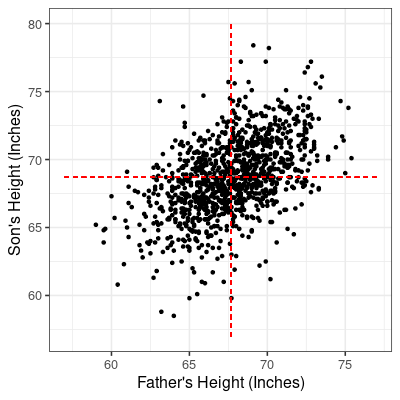
\includegraphics[scale=0.4]{father_son.png}
\end{center}
  \end{column}
\end{columns}
\end{frame}

\begin{frame}{Pearson's Height Data}
We could calculate our regression line using info from this table.

\begin{table}[ht]
\centering
\footnotesize
\begin{tabular}{rccc}
  \hline
& Mean & Std.Dev. & Correlation ($r_{xy}$)\\ 
  \hline
Father & 67.68 & 2.74 & \multirow{2}{*}{0.501} \\ 
Son &  68.68 & 2.81 & \\ 
   \hline
\end{tabular}
\end{table} \vspace{3mm}

\begin{columns}
 \begin{column}{0.45\textwidth}
Regression equation: $\hat{y} = b_0 + b_1X$

\begin{align*}
b_0 & = (\frac{s_x}{s_y})r \\
& = (\frac{2.81}{2.74})0.501 = 0.514
\end{align*}
\begin{align*}
b_1 & = \overline{y}-b_1 \overline{x} \\
& = 68.68 - 0.514*67.68 = 33.893
\end{align*}
 \end{column}
 \begin{column}{0.45\textwidth}
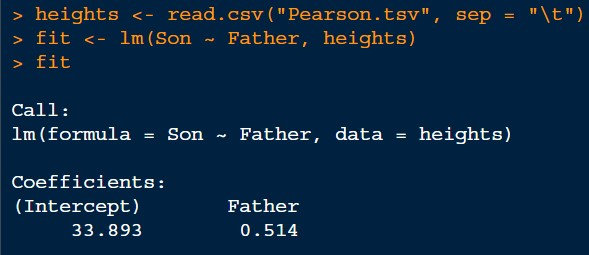
\includegraphics[scale=.55]{img/pearson_heights_regression_coef.jpg}
 \end{column}
\end{columns}
\end{frame}


\begin{frame}{Pearson's Height Data -- Plot Line}
We can make R graph the line on our scatterplot.
\begin{center}
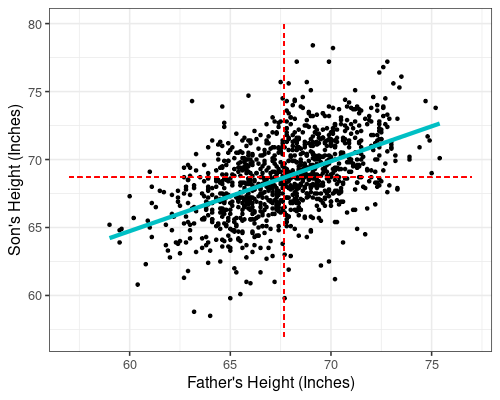
\includegraphics[scale=.5]{img/father_son_lm.png}
\end{center}
\end{frame}

\begin{frame}{Pearson's Height Data -- Prediction}
\footnotesize
The formula for the regression line
\begin{align*}
\hat{y} &= b_0 + X b_1
\end{align*}
can be expressed in terms our our original variables and what we wish to predict
\begin{align*}
\widehat{\text{Son's Height}} &= 33.9 + 0.51 \times \text{Father's Height}
\end{align*} \vspace{6mm}

\textit{Given} the Father's height, we can predict the son's height using this equation by plugging in a value for the father's height \vspace{3mm}

\textbf{Example}: Predict the height of the son for a father with a height of 65in. \vspace{3mm}

\begin{align*}
\widehat{\text{Son's Height}} &= 33.9 + 0.51 \times 65.0 = 67.30in.
\end{align*}

\end{frame}

\begin{frame}{Pearson's Height Data -- Prediction}
Predicted Son's Height = 67.30 inches for a father with height = 65in
\begin{itemize}
    \item Check to see if our prediction makes sense on the graph
\end{itemize}
\begin{center}
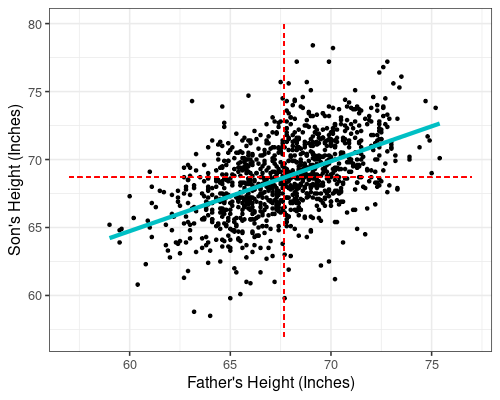
\includegraphics[scale=.5]{img/father_son_lm.png}
\end{center}
\end{frame}


\begin{frame}{Residual}
A \textbf{Residual} is the difference between an observed value and a prediction

\begin{itemize}
    \item often labeled as \textbf{e} \hspace{2mm}("error", r is taken)
    \item e = y - $\hat{y}$
\end{itemize} \vspace{6mm}

\textbf{Interpretation}: the residual tells us whether we have over- or under-predicted the values for the response variable in our data (and by how much)
\begin{itemize}
    \item positive value $\rightarrow$ under-predicted
    \item negative value $\rightarrow$ over-predicted
\end{itemize}
    
\end{frame}



\begin{frame}{Pearson's Height Data -- Residual}
In our data set, the first father had a height of 65 inches. We can calculate the residual for this father. We predicted the son's height to be 67.30 inches.
    \begin{columns}

  \begin{column}{0.5\textwidth}
\begin{align*}
    e & = y - \hat{y}\\
    & = \text{observed value - predicted value}\\
    & = 59.8in. - 67.30in. = -7.5 in.
\end{align*} \vspace{3mm}

\textbf{Interpretation}: We overpredicted the height of this particular son by 7.5 inches  
  \end{column}
  
  \begin{column}{0.3\textwidth}
\begin{center}
\begin{table}[ht]
\centering
\begin{tabular}{rr}
  \hline
Father & Son \\ 
  \hline
65.0 & 59.8 \\ 
  63.3 & 63.2 \\ 
  65.0 & 63.3 \\ 
  65.8 & 62.8 \\ 
  61.1 & 64.3 \\ 
  63.0 & 64.2 \\  
  \vdots & \vdots \\
   \hline
\end{tabular}
\end{table}
\end{center}
  \end{column}
\end{columns}
\end{frame}



\begin{frame}{Slope Interpretation}
Regression equation: $\hat{y} = b_0 + b_1X$ \vspace{2mm}

The \textbf{slope} ($b_1$) tells us how our predictions change when we use different values for the explanatory variable. \vspace{4mm}

\par\noindent\rule{\textwidth}{0.5pt}

\textbf{Interpretation 1}:

For each 1 unit change in the explanatory variable (x), the predicted value of the response variable (y) will change by [value of slope]. \vspace{3mm}

\textbf{Interpretation 2}:

For each 1 unit change in the explanatory variable (x), the value of the response variable (y) will change by the [value of slope], on average.

\end{frame}

\begin{frame}{Intercept Interpretation}
Regression equation: $\hat{y} = b_0 + b_1X$ \vspace{2mm}

The \textbf{intercept} ($b_0$) is the value where our line crosses the y-axis. \vspace{10mm}


\textbf{Interpretation}: When the explanatory variable (x) is zero, we predict the response variable (y) to have a value of [intercept value]. \vspace{6mm}

\textbf{Ask yourself:} Does the intercept interpretation make sense?
\begin{itemize}
    \item Is the intercept value actually possible for our response variable?
    \item Does it make sense to make a prediction using zero for the explanatory variable?
\end{itemize}
\end{frame}

\begin{frame}{Pearson's Height Data -- Interpretations}
    \begin{align*}
\widehat{\text{Son's Height}} &= 33.9 + 0.51 \times \text{Father's Height}
\end{align*}

\textbf{Slope Interpretation:} 

For each 1 inch change in Father’s height, the prediction for son's height changes by 0.51 inches.

-OR-

For each 1 inch change in Father’s height, the son's height changes by 0.51 inches, \textit{on average}. \vspace{4mm}

\textbf{Intercept Interpretation:}

When the father's height is zero inches, the predicted height for the son is 33.9 inches.
\begin{itemize}
    \item does this make sense?
\end{itemize}
\end{frame}

\begin{frame}{Intercept and Extrapolation}

\begin{columns}

 \begin{column}{0.45\textwidth}
\footnotesize
\begin{align*}
\widehat{\text{Son's Height}} &= 33.9 + 0.51 \times \text{Father's Height}
\end{align*}
\begin{center}
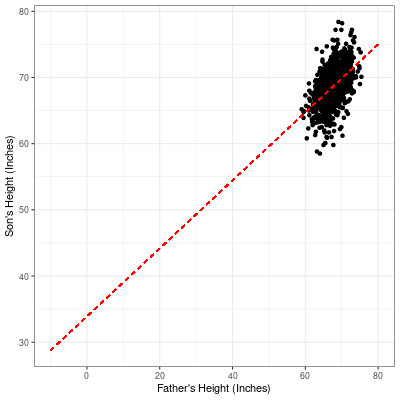
\includegraphics[scale=0.4]{father_son3.png}
\end{center}
 \end{column}
 \begin{column}{0.45\textwidth}
\textbf{Extrapolation} means making predictions for values outside of our data
\begin{itemize}
    \item These predictions are unreliable, since we don't know if the relationship is true for these values
\end{itemize}
 \end{column}
\end{columns}
\end{frame}



\begin{frame}{Extrapolation}
\footnotesize
In 2004, an article was published in \textit{Nature} titled ``Momentous sprint at the 2156 Olympics." The authors plotted the winning times of men's and women's 100m dash in every Olympic contest, fitting separate regression lines to each; they found that the two lines will intersect at the 2156 Olympics. Here are a few of the headlines: \\
\vspace{3mm}
\begin{itemize}
\item ``Women `may outsprint men by 2156'" -- BBC News
\item ``Data Trends Suggest Women Will Outrun Men in 2156" -- Scientific American
\item ``Women athletes will one day out-sprint men" -- The Telegraph
\item ``Why women could be faster than men within 150 years" -- The Guardian
\end{itemize}


\end{frame}

\begin{frame}
\begin{center}

\includegraphics[scale=0.25]{nature_headline.png}
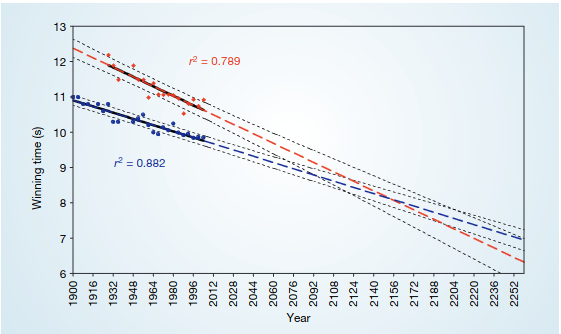
\includegraphics[scale=0.5]{nature_plot.png}
\end{center}
\end{frame}

\begin{frame}{12 years of data later}
\begin{center}
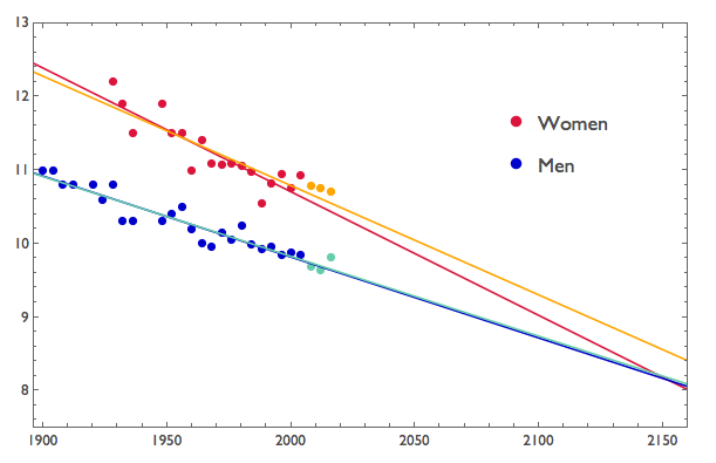
\includegraphics[scale=0.4]{nature_update.png}
\end{center}
\end{frame}

\begin{frame}{Asymmetry}
Unlike correlation, where $r_{xy} = r_{yx}$ (whether you put the variables on the x- or y-axes doesn't matter) regression is \textit{asymmetrical}: the choice of explanatory and response variables matter for the line
\begin{center}
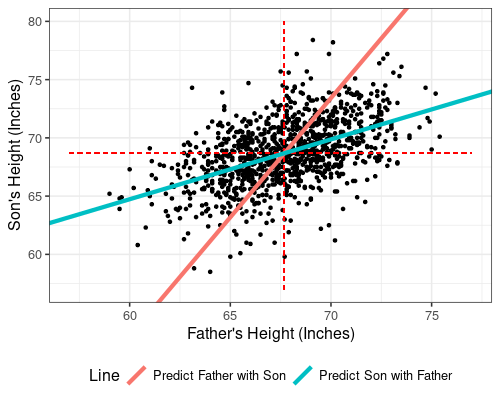
\includegraphics[scale=0.45]{father_son_lm2.png}
\end{center}
\end{frame}



\begin{frame}{Assessing Quality of Fit}
\small
The less variability there is for the points around the regression line, the better the line fits the data. (More variability $\rightarrow$ worse fit)

\begin{center}
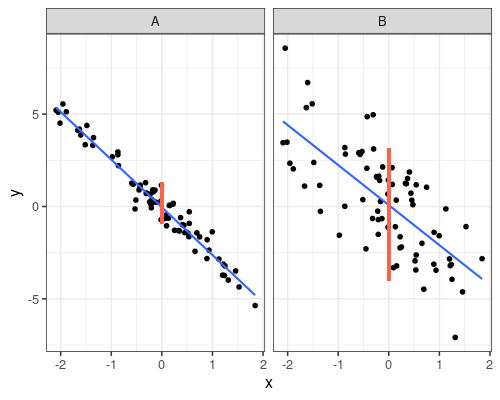
\includegraphics[scale=0.5]{qof2.png}
\end{center}
\end{frame}

\begin{frame}{Assessing Quality of Fit}
    With this in mind, we can quantify how well the line fits the data using: \vspace{3mm}

\textbf{Coefficient of determination} ($R^2$)
\begin{itemize}
    \item measures how close the observations match the predictions
\begin{align*}
    R^2 = \frac{\text{variance of predicted y's}}{\text{variance of observed y's}} = \frac{s_{\hat{y}}^2}{s_y^2}
\end{align*}

\item ratio written as decimal or percentage between 0$\%$ and 100$\%$
\item larger values indicate better fit, stronger linear relationship between the variables
\end{itemize} \vspace{3mm}

\textbf{Interpretation:} 

$R^2$ is the percentage of variation in the observed values of the response variable (x) that can be explained with the linear regression model including the explanatory variable (y). [include context]

\end{frame}


\begin{frame}{Assessing Quality of Fit}
We also saw that the \textbf{correlation coefficient (\textit{r})} can be used to quantify the strength of the linear relationship. \vspace{3mm}

There is a connection between r and $R^2$.
\begin{itemize}
    \item $r^2 = R^2$
    \item r = $\pm \sqrt{R^2}$ \hspace{2mm} (need to find the correct sign using scatterplot / slope)
\end{itemize}
\end{frame}

\begin{frame}{$R^2$ Interpretation}
    The correlation coefficient for the Pearson Height data is r = 0.501
\begin{align*}
    R^2 = r^2 = .501^2 = 0.251
\end{align*} \vspace{3mm}

\textbf{Interpretation}:
"25.1$\%$ of the variation in son's height can be explained using our linear regression with father's height as the predictor." \vspace{3mm}

$\rightarrow$ 25.1$\%$ of the differences in height for sons is because of the their father's height. 74.9$\%$ of their differences in height is because of other stuff

\end{frame}






\begin{frame}{Review}
We should be able to 

\begin{itemize}
\item Use a line to describe a linear relationship
\item Be able to predict an outcome, given a predictor
\item Interpret the slope (and intercept if applicable)
\item Assess the quality of a fitted line using $R^2$
\end{itemize}
\end{frame}


%
%
%\begin{frame}{Regression with Categorical Predictors}
%Predict enrollment from private or public \\
%
%indicator variables
%
%bonus intercepts not slopes
%\end{frame}
%
%\begin{frame}
%another example looking at enrollment by region, what is reference var, see it's like conditional mean, i.e., given x here is y except one continuous and one discrete
%\end{frame}
%

%%%%%%%%%%%%%%%%

%\begin{frame}
%\begin{columns}
%
%  \begin{column}{0.45\textwidth}
%%
%  \end{column}
%  \begin{column}{0.45\textwidth}
%%
%  \end{column}
%
%\end{columns}
%\end{frame}


\end{document}
